A full spectrum of different techniques can potentially be used. Grasping the theory behind these various techniques is primordial when making decisions to establish the requirements and conceptualise the design. Therefore, this chapter will study the literature surrounding three crucial areas that are necessary to understand what is required for a content-based video retrieval system targeting long videos.\\

The first section will address general content-based retrieval systems concepts, retracing the evolution of such systems for videos and addressing the challenges posed by targeting a content-based retrieval system for videos and recording queries through mobile devices. The second section will focus on extracting visual content from videos, starting with the different types of static features and ending with dynamic features. Finally, the third section targets how the structure of videos can be used to segment and extract individual frames to densely represent them in order to optimise the system.

%%%%%%%%%%%%%%%%%%%%%%%%%%%%%%%%%%%%%%%%%%%%%%%%%%%%%%%%%%%%%%%%%%%%%%%%%%%%%%%%%%
% 1 - CONTENT-BASED RETRIEVAL 
%%%%%%%%%%%%%%%%%%%%%%%%%%%%%%%%%%%%%%%%%%%%%%%%%%%%%%%%%%%%%%%%%%%%%%%%%%%%%%%%%%
\section{Concepts Behind a Content-Based Video Retrieval System}

Content-based retrieval is a type of visual search technique where large databases of either images or videos are queried to find the closest match to a query image or video. Although this project focuses on content-based video retrieval, also referred to as CBVR\footnote{Content-Based Video Retrieval}, image retrieval techniques (CBIR\footnote{Content-Based Image Retrieval}) will be discussed as well due to their relevance in video retrieval.\\

This section will first review the different video retrieval methods and their evolution, starting from text-based retrieval to content-based retrieval, before addressing the various challenges that exist in video retrieval, such as the additional difficulty caused by the temporal aspect of videos compared to images, and the complications of targeting mobile devices for such a system.

% ----------------------------------------------------

\subsection{Video Retrieval Methods}
\label{sec:cbvr-methods}

Drastic advances in video capturing technology have caused important amounts of unstructured data in the form of videos to be produced in recent years. This has lead to a high-demand to develop new efficient solutions for processing this data, with video retrieval being the answer.\\

Throughout the years, video retrieval has improved in parallel with the breakthroughs in video recording devices. Early video retrieval techniques used a text-based approach where the system accepted text input to search the database of videos \cite{lai2015trajectory}, as seen in Figure \ref{fig:text_vs_content_retrieval}.\emph{a}. For example, the user would input the string query \textit{``De Niro''}, which would return all movies in which Robert De Niro starred or \textit{``Coppola''} to find all movies directed by Francis Ford Coppola. Unique aspects of the video clip such as movie credits or sports scores were often analysed using OCR\footnote{Optical Character Recognition} technology \cite{li2002text}. The query text was then compared to a video file's content, such as colours, shapes, texture, luminance or objects, or to the file's metadata\footnote{The data associated to a video file}, such as the video title, author, date, content description, commentaries, captions or keywords \cite{li2002text} \cite{feng2011} \cite{patel2012}. However, these techniques were highly inefficient compared to content-based techniques as they often relied on manually noted annotations and textual descriptions to find similarities for matching the query video to a video in the database and did not make use of the actual visual content that describes a video.\\

\begin{figure}[h]
\centerline{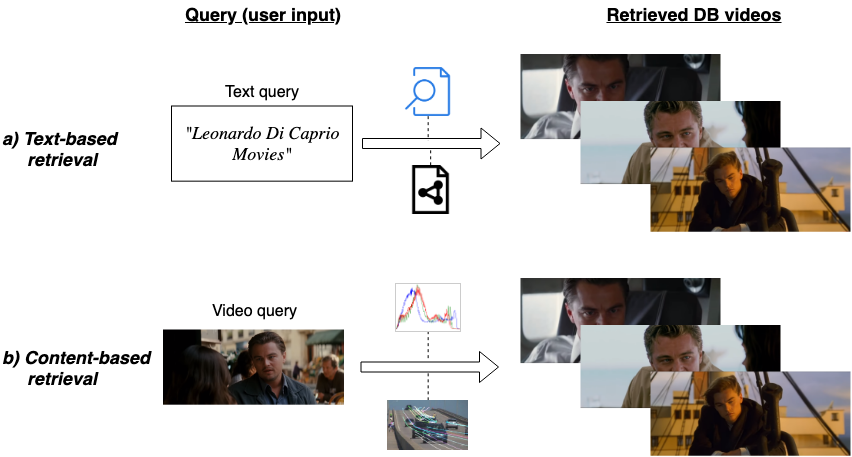
\includegraphics[width=\textwidth]{figures/litsurvey/content_text-retrieval_comparison.png}}
\caption{\label{fig:text_vs_content_retrieval}Illustrations of a text-based content-retrieval system \emph{(a)} and a content-based video retrieval system \emph{(b)}.}
\end{figure}

Content-based retrieval techniques quickly replaced text-based retrieval techniques towards the end of the 20th century by making use of the visual content to compute similarities between videos \cite{lai2015trajectory}. Instead of accepting a text string, the system takes a video as input to extract its visual contents, as shown in Figure \ref{fig:text_vs_content_retrieval}.\emph{b}. According to Petković et al. \cite{petkovic2000}, this visual content can be broken down into three different categories:
\begin{itemize}
    \item \textit{Raw data}, which corresponds to individual raw video frames and the video file's attributes such as the frame rate per seconds, the number of bits per pixel or the colour model used.
    \item \textit{Low-level visual content}  consists of the visual features that describe a video. This content includes colours, shapes, textures and motion. Low-level visual content can be extracted into static features such as histograms (see Section \ref{sec:color-based-features}) or dynamic features such as objects or motion (see Section \ref{sec:dynamic-features}) using a wide variety of existing techniques. Once the content has been extracted, it can be used to first compute similarities between videos \cite{lai2015trajectory} and later pattern match them.
    \item \textit{Semantic content} contains the high-level concepts that are present in a video. These high-level concepts can be described as objects or events using the features. To extract semantic content from a video, a grammar of rules for objects must be provided. An example of an object rule could be ``if the shape is round, the colour is orange and the object is moving, then that object is a basketball''.
\end{itemize}

In comparison to raw data, low-level visual content provides the most relevant visual information that can be extracted from a video for the purpose of a CBVR system. Semantic content extraction adds an additional layer of complexity compared to low-level visual content extraction as it requires domain knowledge and user interaction \cite{petkovic2000}. Therefore, this project will focus on using low-level visual content to extract information about the video and compute the similarities between the query video and database videos. It is important to note that this project's goal differs from classic CBVR systems where a list of videos is returned (see in Figure \ref{fig:text_vs_content_retrieval}.\emph{b}), as it must return a specific video that matches the most the query video. To improve the pattern matching accuracy phase, raw data (e.g. audio) and metadata (e.g. captions) may be used to improve the pattern matching accuracy \cite{patel2012}.\\

% ----------------------------------------------------

\subsection{Temporal Aspects of Videos}
\label{sec:temporal-aspect-videos}

\subsubsection{Temporal Structure of a Video}

The most important difference between content-based image retrieval and video retrieval lies within the temporal aspect of the video. Naturally, the temporal aspect of a video clip stores supplementary information about the content, including dynamic low-level visual content e.g. an object's motion, and semantic content e.g. actions and events. According to A. Araujo et al. \cite{araujo2017i2v}, a video's temporal structure can be subdivided into three units, as shown in Figure \ref{fig:temporal_structure}:
\begin{itemize}
    \item \textit{Frames} correspond to the smallest temporal unit of a video file. A single segment of a video is referred to as a frame. Frames are also used to describe the frame rate (the frequency at which consecutive stills appear on a screen every second) e.g. ``24 fps'' corresponds to a video made up of 24 stills per second.
    \item \textit{Shots} are grouped sequences of visually similar frames. They are usually described in seconds.
    \item \textit{Scenes} are collections of shots which are related based on the action and objects present in the shot, thus giving them a semantic aspect. The length of a scene is generally calculated in minutes rather than seconds.
\end{itemize}

\begin{figure}[h]
\centerline{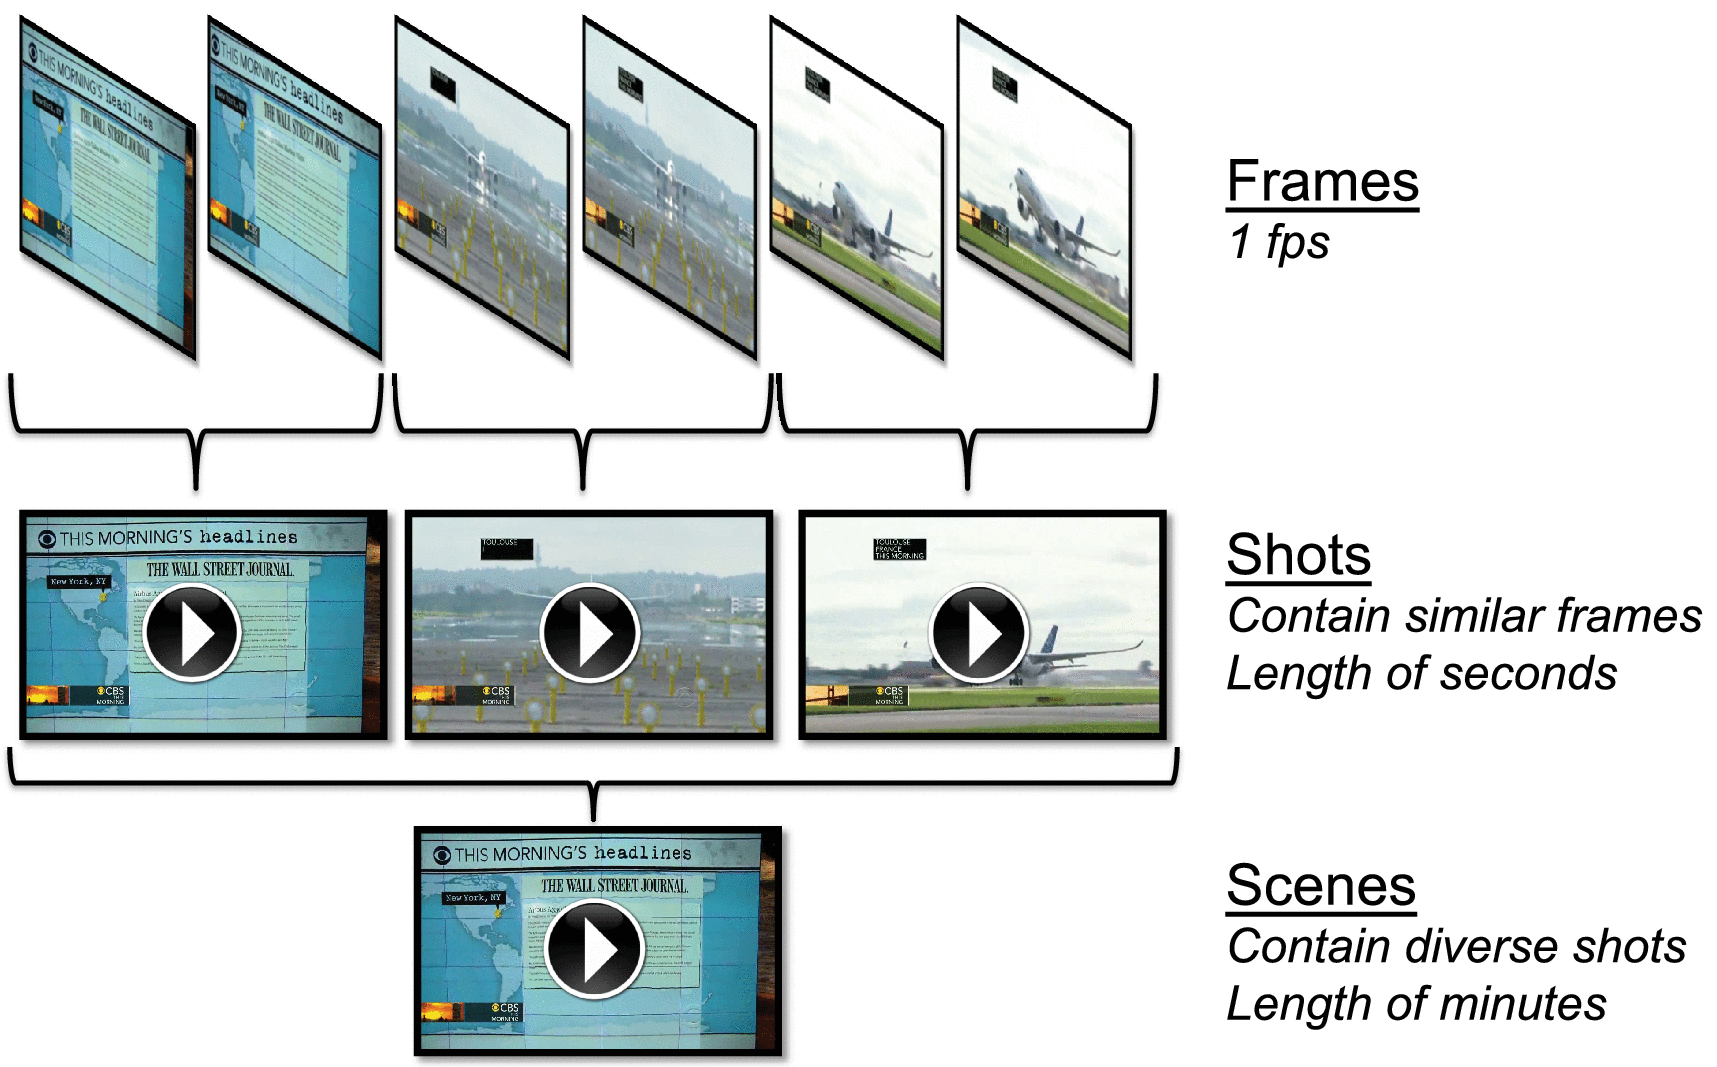
\includegraphics[width=0.75\textwidth]{figures/litsurvey/temporal_structure_videos.png}}
\caption{\label{fig:temporal_structure}Temporal structure of videos, including the different terms used to describe video temporal units. Figure courtesy of A. Araujo et al.}
\end{figure}

Because this project will explore possible solutions to create a CBVR system targeting databases of feature-length movies, a fourth video temporal structure category relevant to this project can be added to Araujo et al.'s initial list:
\begin{itemize}
    \item \textit{Movies} can be described as a large group of scenes that are used to tell a story. Movie durations commonly range from one to three hours.
\end{itemize}

\subsubsection{Challenges of Temporality}
\label{sec:litsurvey-challenges-temporality}

Multiple challenges arise when dealing with CBVR systems in contrast to CBIR systems as the videos' temporal aspect adds a new dimension of complexity when extracting visual information. While the low-level visual content describing images remains mostly the same for videos, some new information that did not exist in images can be extracted, such motion. As mentioned previously, videos are made up of frames, which make up shots when a combination of similar frames are played in succession. This means that videos carry information about motion, such as the trajectory of objects. This introduces unique challenges to the algorithms used to extract motion.\\

Because videos are made up of numerous stills, usually around 24 frames per second \cite{brownlow1980silentfilm}, two consecutive frames are near-identical. The pixels describing an object in one frame will remain the same in the next frame, except for the edge pixels perpendicular to the motion's trajectory \cite{bradski2008opencv}.\\

Figure \ref{fig:forrest_gump_frames} shows six frames from Forrest Gump's famous running shot, which lasts 44 seconds, making up a total of 1056 frames. Each frame in the figure was captured with 10-second intervals, meaning 240 frames separate each still. In the first three frames, the group of people running in the background barely moves in the space of 20 seconds. The pixels that describe the group in the shot remain mostly unchanged for all of the frames between the 3 samples, equivalent to 480 frames, with a few additional pixels describing the group as it advances towards the camera. The same can be said about the red cap in the last two frames. Most of the pixels making up the cap in the fifth frame remain the same in the sixth frame. This example perfectly betrays the reason why analysing a video frame by frame would be extremely inefficient when it comes to CBVR. Due to the similarities between consecutive frames, these should be aggregated \cite{araujo2017i2v} to describe a shot by using a selection of frames, such as taking the six frames in Figure \ref{fig:forrest_gump_frames} to describe the entire 44 seconds of video, rather than keeping the original 1056 frames to describe it.

\begin{figure}[h]
\centerline{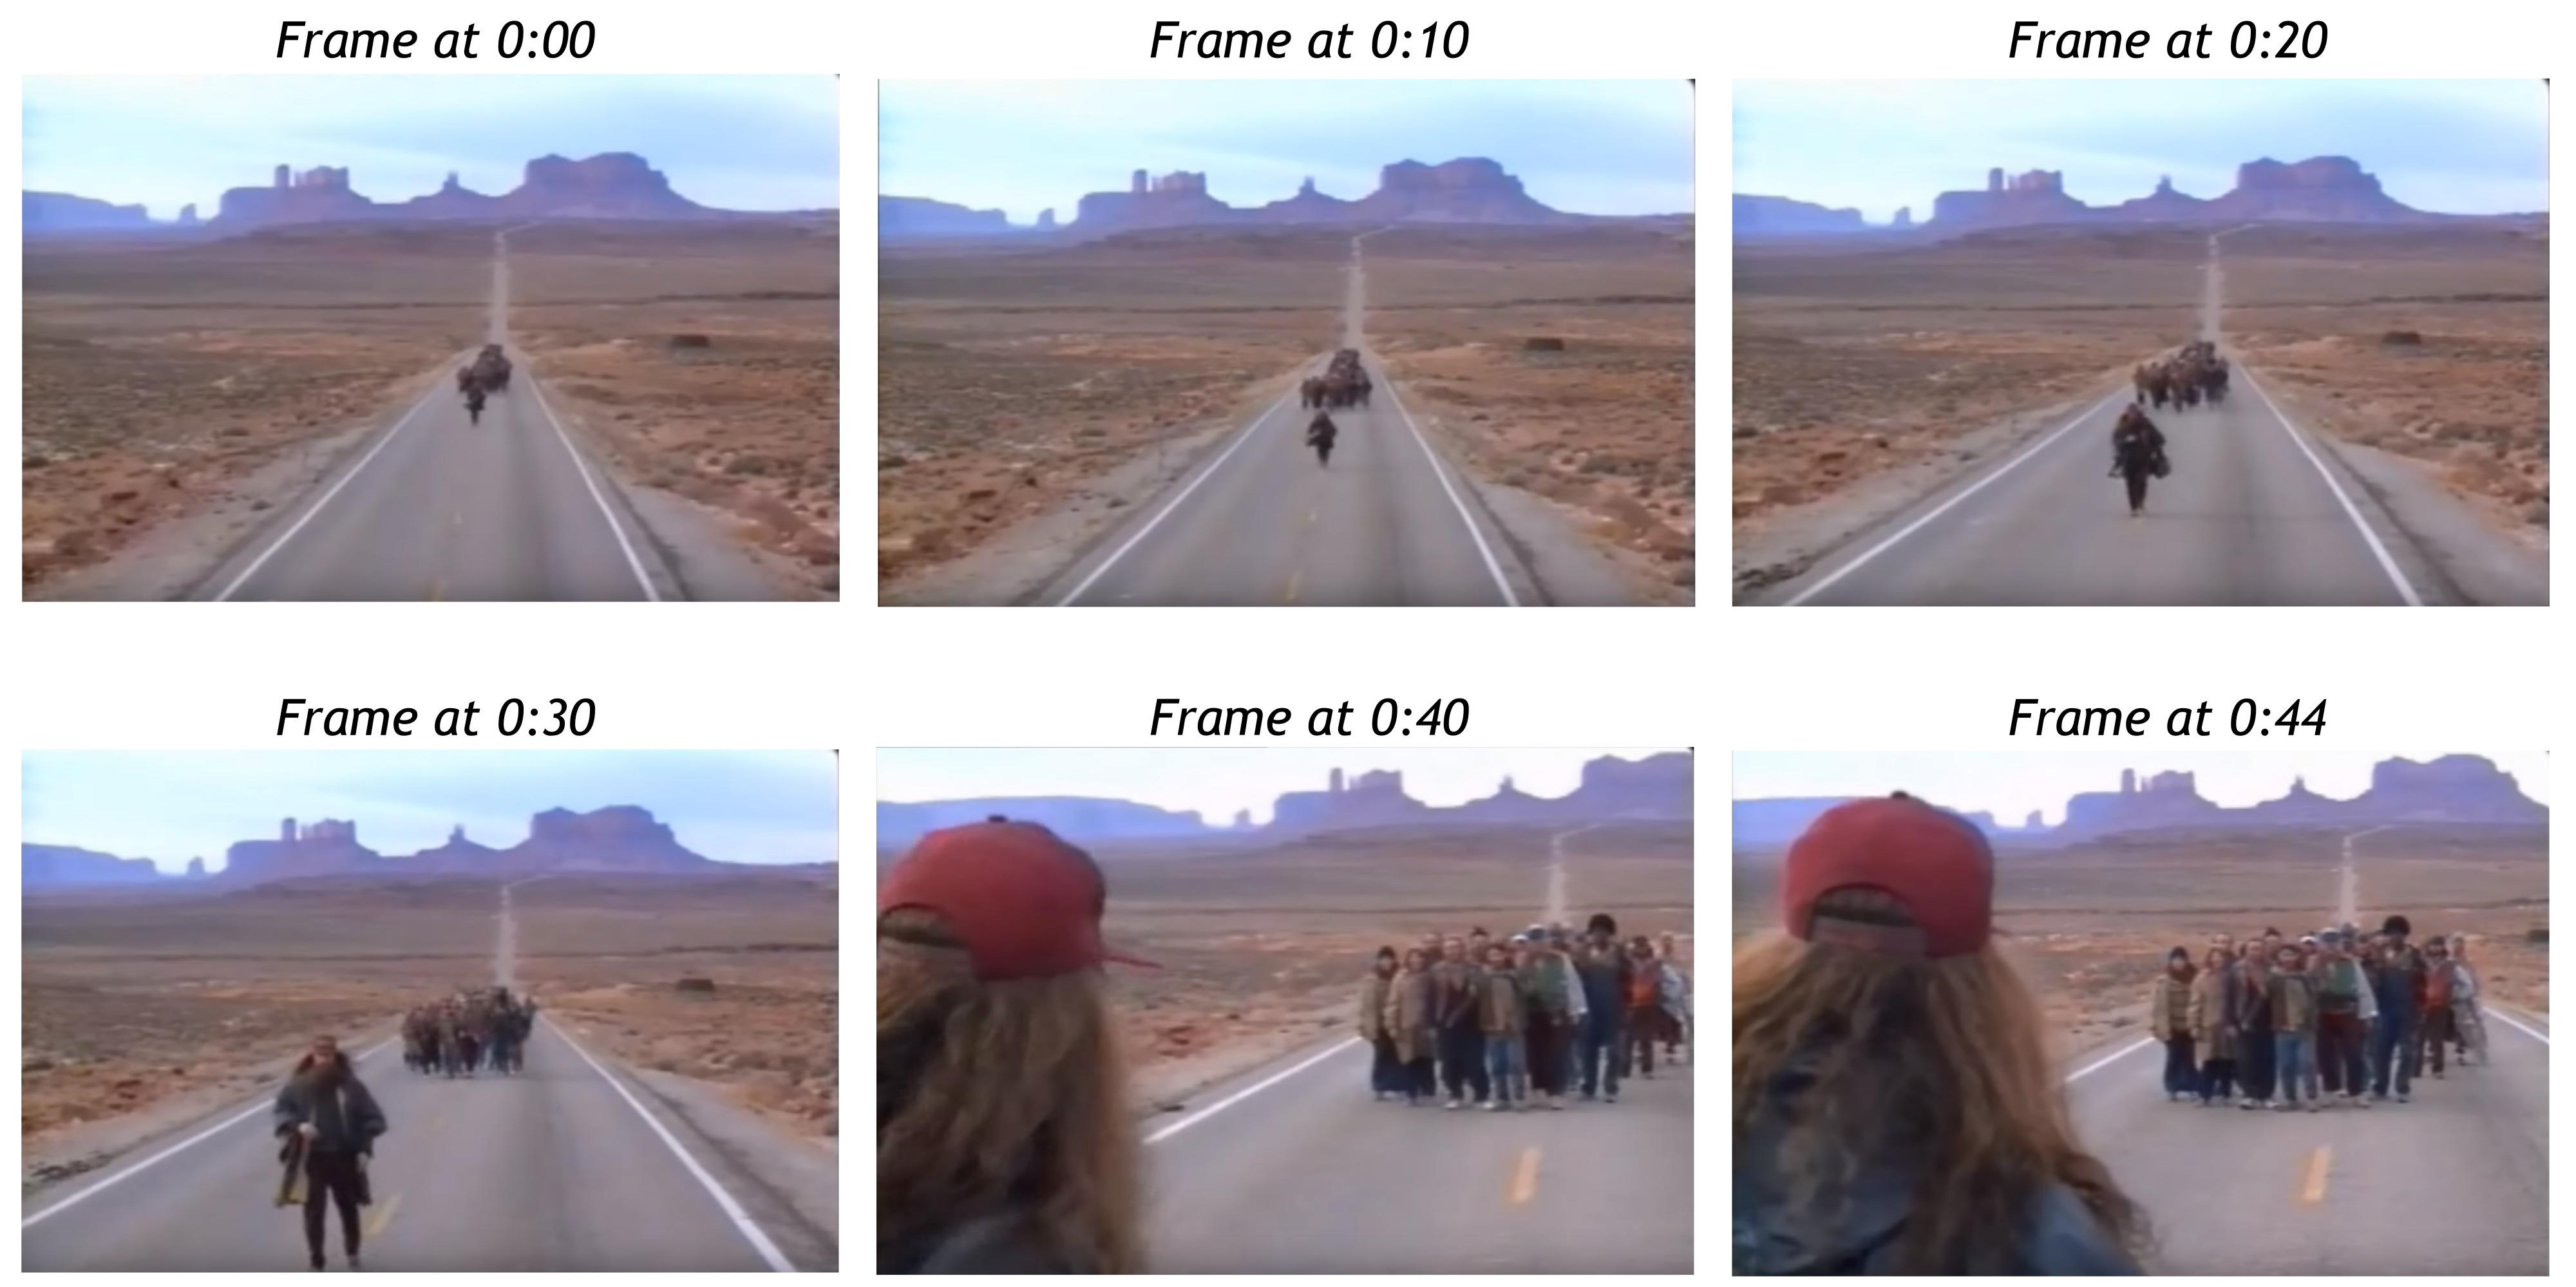
\includegraphics[width=\textwidth]{figures/litsurvey/forrest_gump_shot.jpg}}
\caption{\label{fig:forrest_gump_frames}Frames from the famous running scene in Forrest Gump extracted at intervals of 10 seconds. Video frames courtesy of \textit{``Forrest Gump long run scene''} YouTube video available online: \url{https://youtu.be/QgnJ8GpsBG8?t=325}.}
\end{figure}

\begin{comment}
    On top project aim mobile device using a database of feature-length movies.\\
    \cite{araujo2017i2v}One of the problems regarding video retrieval is the temporal aspect of the data. A solution to overcome the temporal aspect of the data is to aggregate each video into a compact signature to allow quicker and more efficient matching (when matching the query video to a video in the database).\\ 
    temporal aggregation problem of videos compared to images
\end{comment}


\subsection{CBVR for Mobile Devices}
\label{sec:litsurvey-cbvr-4-mobile-devices}

The aforementioned project aim is for the system to work on mobile devices for two reasons. The first reason is to allow users to directly use their mobile phone to record the query video by pointing their camera to a screen displaying a movie, which will, in turn, tell them which movie is being played (see the wireframe in Figure \ref{fig:wireframe}). Additional information retrieved from IMDb\footnote{Internet Movie Database}, such as cast, crew, ratings, runtime and synopsis could also be displayed. The second reason is the popularity of mobile devices, which may be due to the improvements made on mobile phones' processing power, allowing more tasks to be carried out through this medium. However, such a system on a mobile device causes many problems regarding the query video recording method and the computational power available on mobile devices.\\

\subsubsection{Query Video Quality}

Large visual differences are caused between the query clip and the actual clip stored in the database due to the capture conditions \cite{liu2014mobilevideosearch} \cite{wang2016actionregonition} such as:
\begin{itemize}
    \item Undesired camera movements due to unstable recording e.g. unstable recording, hand shaking.
    \item Low-quality recording due to poor user recording e.g. scaling and rotation, and due to the environmental conditions e.g. lighting, reflections, blurring.
    \item Video noise because of the camera sensor.
    \item Decoding artefacts caused by various file compression.
\end{itemize}

These low-quality conditions add difficulty to the pattern matching phase where the similarities between the query video and database videos have to be computed. Indeed, if the query video is very different from the actual video, then the noisy elements of the video query must be filtered out. For example, if the recorded video is shaky, then this shaking motion has to be pruned before analysing the recorded clip's motion. However, processing power must be used from the actual visual content extraction and pattern matching phases to be used for video noise filtering.

\subsubsection{User Experience}

According to Liu et al. \cite{liu2014mobilevideosearch}, the majority of mobile device users expect a polished product with quick video query and instant or progressive results, meaning that the searching algorithms must be efficient. However, one of the downsides of mobile devices is the computation power constraints. Despite the improvements in mobile processors, desktop devices still remain more powerful than mobile ones. A solution that Liu et al. suggest is to retrieve the low-level visual content locally on the mobile device and send the query to a server where the pattern matching will take place \cite{liu2014mobilevideosearch}. This allows heavy computations to be off-loaded from the mobile device. Once a match is found, the result is returned to the user on his mobile device. A downside to this approach is the new constraint on network bandwidth rather than computational power.

\begin{comment}
    % todo - spread in sections above
    \subsubsection{Computational efficiency and database size}
    
    At the early stages of the development phase of the project, the database of videos for the system will be made up of shots only, lasting on average ten seconds. Longer videos will be used progressively based on the system's progress with shorter videos.\\
    mention \cite{hanjalic1999moviesegmentation}
    
    \cite{wang2016actionregonition}
    A challenge also lies within the computational power needed to process all the data in a database efficiently.\\
\end{comment}


%%%%%%%%%%%%%%%%%%%%%%%%%%%%%%%%%%%%%%%%%%%%%%%%%%%%%%%%%%%%%%%%%%%%%%%%%%%%%%%%%%
% 2 - VISUAL CONTENT EXTRACTION
%%%%%%%%%%%%%%%%%%%%%%%%%%%%%%%%%%%%%%%%%%%%%%%%%%%%%%%%%%%%%%%%%%%%%%%%%%%%%%%%%%
\section{Visual Content Extraction for Pattern Matching}
\label{sec:visual-content-extraction}

Extracting the visual content from a video allows this content to be used to describe videos and compute similarities between them. This visual content is extracted from the aforementioned low-level visual content (see Section \ref{sec:cbvr-methods}) \cite{petkovic2000} and stored in the form features, also referred to as visual descriptors. The term ``features'' is very broad and can be used to describe many different visual aspects in an image or in a video, ranging from colours, shapes and textures to points, edges, objects and motion.\\

These features can be divided into two categories: static features and dynamic features \cite{petkovic2000}. This section will first survey examples of static visual descriptors and methods to extract them from videos, and will then focus on examples and methods of extracting dynamic visual descriptors from videos.

% ----------------------------------------------------

\subsection{Static Features}

Methods to extract static features operate on stills, which can correspond to individual video frames, thumbnails or key frames (see Section \ref{sec:movie-pre-processing}). This means that traditional image techniques can be applied to those stills \cite{hu2011survey}. They are organised in three different categories: colour-based features, texture-based features and shape-based features, which can visualised in Figure \ref{fig:colour-texture-shape-features}.

\begin{figure}[h]
\centerline{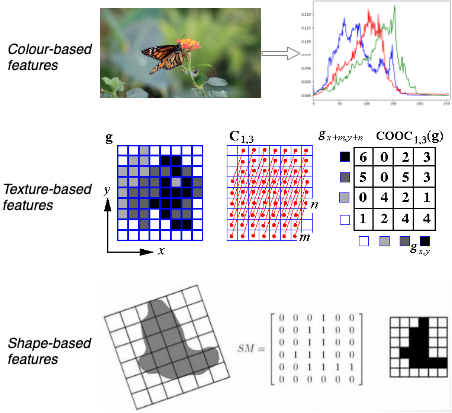
\includegraphics[width=0.75\textwidth]{figures/litsurvey/colour-texture-shape-features.png}}
\caption{\label{fig:colour-texture-shape-features}Example of static features, including colour-based features (with an RGB colour histograms of 256 bins for colour-based features), texture-based features (with an co-occurrence matrix showing the frequency of pairs of pixels) and shape-based features (with a shape matrix descriptor).}
\end{figure}

\subsubsection{Colour-based Features}
\label{sec:color-based-features}

The main colour-based features model are colour histograms. In general, a histogram consists of counts of some underlying data that is organised into predetermined bins to a statistical representation of the distribution of that data. Figure \ref{fig:histogram-general-example} depicts an example of a histogram where a collection of points is organised into specific pre-defined bins based on their location relative to a vertical grid.

\begin{figure}[h]
\centerline{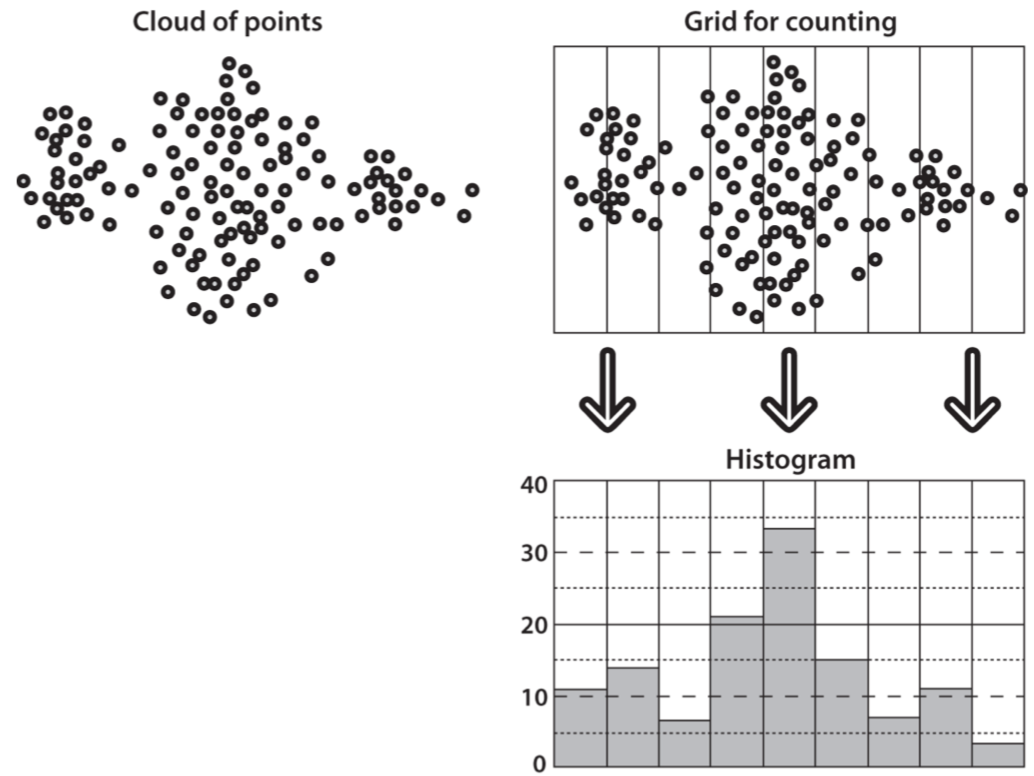
\includegraphics[width=0.75\textwidth]{figures/litsurvey/histogram_general_example.png}}
\caption{\label{fig:histogram-general-example}Example of a histogram counting the location of points relative to a vertical grid. Image courtesy of Bradski and Kaehler.}
\end{figure}

In the case of a colour histogram, the underlying data that the histogram is trying to represent is the distribution of the colour pixels throughout an image or a video frame. Different kinds of colour histograms exist as they depend on the chosen colour space, which includes RGB\footnote{Red Green Blue}, HSV\footnote{Hue Saturation Value}, HSL\footnote{Hue Saturation Light} or YPbPr colour spaces to name a few. These may vary based on the applications of the colour histograms.\\

Typically, for an RGB colour histogram, 256 bins are used to accurately represent all the possible values that the pixels can take (ranging from 0 to 255) for each of the three RGB channels, which are then plotted as three individual graphs. Choosing the right range for the histogram's bins is crucial to represent the distribution efficiently. If the range of pixels that defined the bins is wider, meaning there are less overall bins, then the histogram's distribution would be too coarse-grained and the general structure of the histogram would be lost, as pointed out by the left half of Figure \ref{fig:histogram-bin-size}. On the other hand, if the range of the bins is too narrow, meaning there are more overall bins, then the histogram's distribution would not be represented accurately and there would be many spiky cells, as betrayed in the right half of Figure \ref{fig:histogram-bin-size} \cite{bradski2008opencv}.

\begin{figure}[h]
\centerline{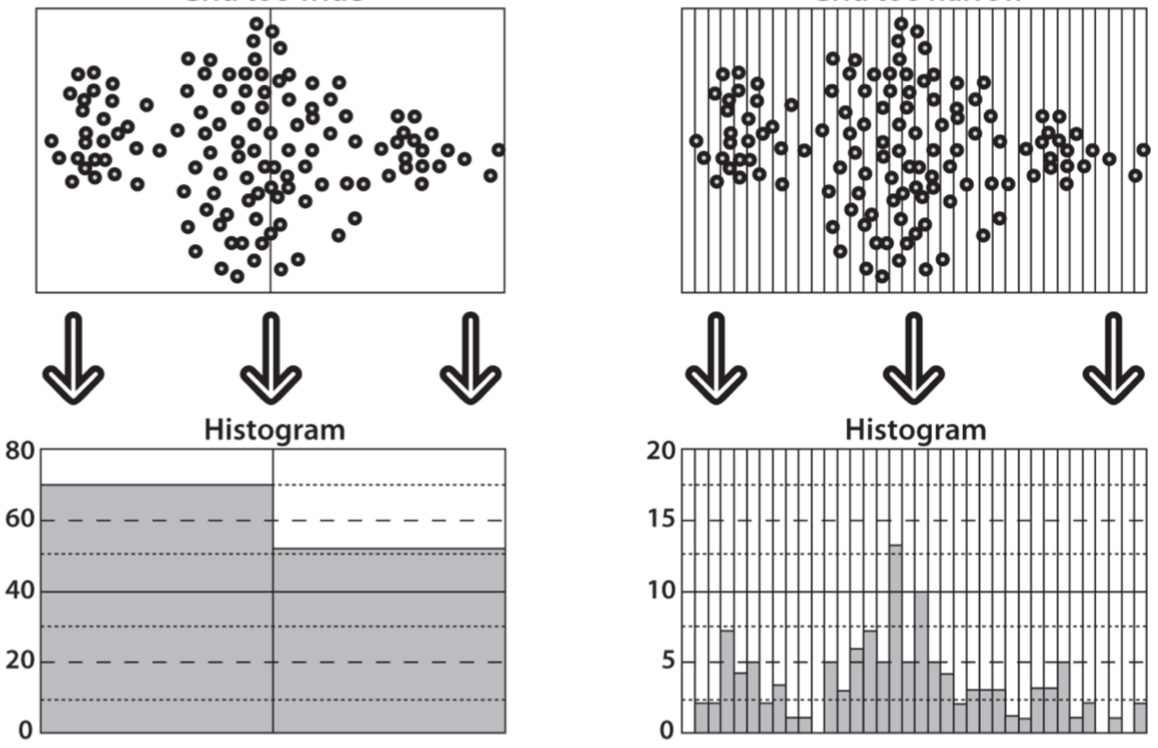
\includegraphics[width=0.85\textwidth]{figures/litsurvey/histogram_bin_size.png}}
\caption{\label{fig:histogram-bin-size}If the range of the bins is too large, then the distribution is coarse (left). If the range of the bins is too small, then the distribution is not accurately represented and spikes cells appear (right). Image courtesy of Bradski and Kaehler.}
\end{figure}

One of the inaccuracies with colour histograms lies within the scope of the distribution. If the histogram represents the global distribution of all the pixels in the still, then two images might have very similar histograms \cite{petkovic2000}. For example, a histogram containing 60\% white pixels and 40\% blue pixels could either describe both a blue sky with white clouds or a snowy landscape with a blue sky. Despite both histograms being good colour-based features, the actual result is still poor when it will be used for matching the histograms. A solution consists in segmenting the still into multiple local images, and extract the local colour-based features for each segment. For example, the still could be partitioned into a 5x5 grid, and a colour histogram could then be computed for each grid \cite{yan2007review}. This would enable colour-based features to represent specific regions of the still rather than globally describing an image. However, the same problem mentioned earlier could occur if the still is segmented into too many regions, causing the overall histogram to be coarse.\\

Other types of colour-based features can be extracted from images and videos such as colour moments, colour correlograms \cite{huang1997correlograms} and Gaussian models. However, colour-based features have their limitations as they cannot describe textures and shapes, rendering them inefficient in certain applications \cite{hu2011survey}.

\subsubsection{Texture-based Features}

Texture-based features are often used in parallel with colour-based features. The aforesaid problem where two different objects might share a similar histogram can be solved by using texture-based features to differentiate them e.g. green tree leaves and green grass. These can be discerned by using a variety of features such as Tamura features, which extract information including coarseness, contrast, and directionality of the objects \cite{amir2003ibm}. 

\subsubsection{Shape-based Features}

Shape-based features are used to describe the overall shape of objects present in the image. The most common approach consists in computing an EHD\footnote{Edge Histogram Descriptor}, which consists in detecting the edges present in the image (see Section edges) and then plot their spatial distribution in a histogram by counting the number of pixels for each edge \cite{hauptmann2004informedia}. The same image segmentation technique can be used to localise the EHD. These shape-based features have many applications but are harder to extract and require more computing power than colour-based features and texture-based features.

% ----------------------------------------------------

\subsection{Dynamic Features}
\label{sec:dynamic-features}

In contrast to static features, which can be extracted from individual video frames, dynamic features require the continuity between consecutive frames to extract relevant visual descriptors, making use of the temporal aspect of the video mentioned in section \ref{sec:temporal-aspect-videos}). These features can be divided into two subcategories: object features and motion features. However, before reviewing the techniques used to extract these features, it is important to specify what defines a good visual feature.

\subsubsection{Points of Interest}

Figure \ref{fig:monaco_palace_features} shows an image with coloured windows used to make the difference between poor and good potential features that could be used for object and motion features:
\begin{itemize}
	\item \textit{Flat surfaces} are portrayed in blue in Figure \ref{fig:monaco_palace_features}. These blue windows are spread over large areas of the image, meaning it is difficult to find their specific location. Moving the blue window along the image in any direction will result in the same visual content being represented in the window. Therefore, these flat regions are the worst structures as they do not contain any useful information.
	\item \textit{Edges} are characterised in green in Figure \ref{fig:monaco_palace_features}. These are more informative than flat surfaces as they can be more accurately localised, but pinpointing an exact location is still hard as the patch can be moved in the direction parallel to the edge. Moving the green window along the edge will again result in the same visual content being represented in the window. Edges are efficient to detect object boundaries, but not for tracking specific points.
	\item \textit{Corner} are characterised in red in Figure \ref{fig:monaco_palace_features}. These are the most descriptive points as they are often unique and can be precisely located in an image. Moving the red window in any direction will cause it to look different. Corners are therefore the ideal candidate for features used in object matching and tracking.
\end{itemize}

\begin{figure}[h] 
\centerline{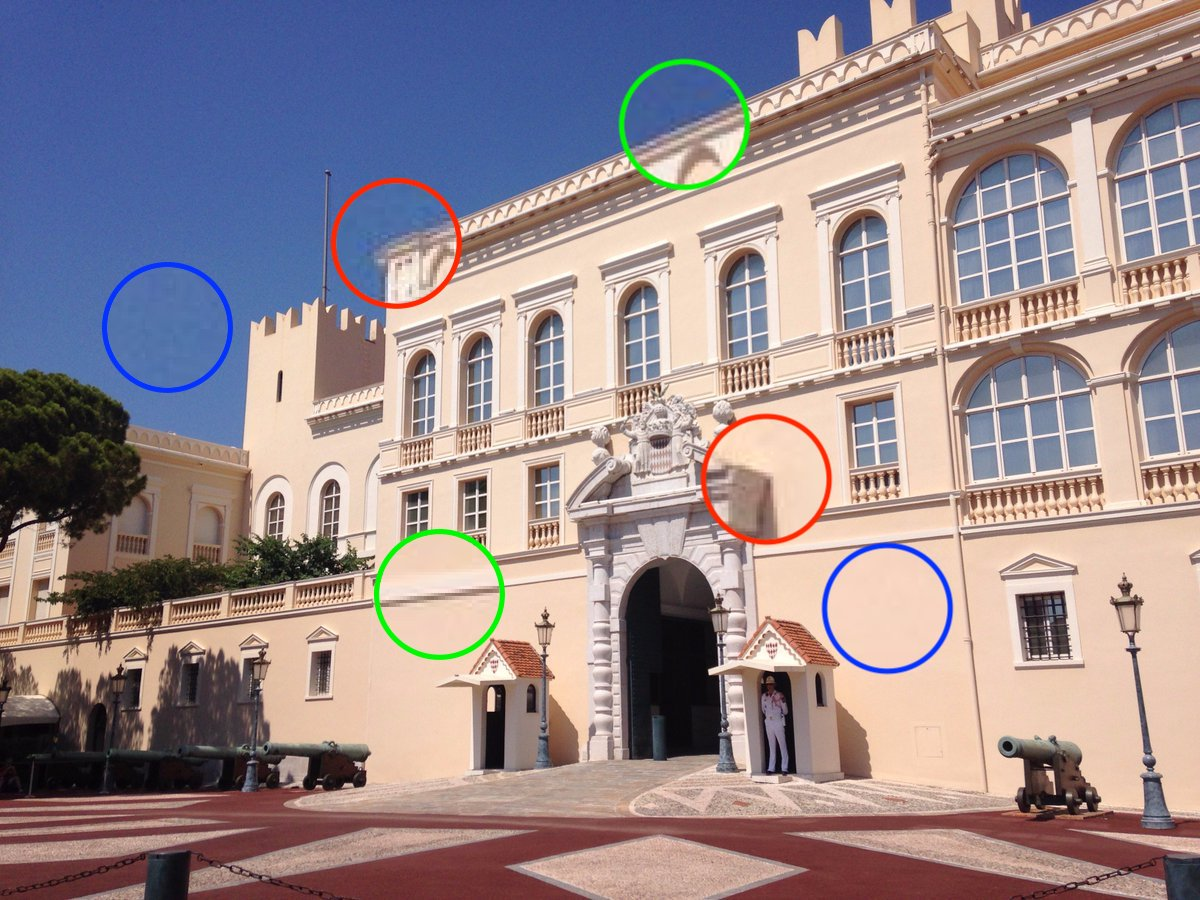
\includegraphics[width=0.80\textwidth]{figures/litsurvey/monaco_palace_features.jpg}}
\caption{\label{fig:monaco_palace_features}An image of the Palace of Monaco with coloured windows representing poor features in blue (flat), edges in green, and good features in red (corners).}
\end{figure}

Once expressive and unique descriptors like corners are detected, they can be used to extract object features and motion features, and to compute similarities between the query video and the videos in the database.\\

Many different algorithms exist to find robust features and interest points. For example, Sobel operators can be used to detect edges, and Shi and Tomasi algorithms and Harris operators can be used to detect corners \cite{bradski2008opencv}. Combinations of both can be used, by detecting edges to facilitate corner detection.

\subsubsection{Object Features}

Object features correspond to objects that are detected using the colour, texture and size of image regions. Some of the most common objects usually detected in videos are faces, as many CBVR systems use them to compute similarities between videos \cite{sivic2005face}. However, extracting object features is time-consuming and expensive in terms of required processing power, which is why CBVR algorithms either focus on detecting specific sets of objects rather than general objects that may be present in a scene, or on static features.

\subsubsection{Motion Features}

Motion features are a unique characteristic of videos that are absent from images. All of the above-mentioned features can be extracted from images, apart from motion features, which are unique to videos. These can originate from two sources: either background camera movement or foreground object movement. Motion features can therefore be classified into two categories: camera-based motion features and object-based motion features. \textit{Camera-based motion features} include movement such as camera zooms, pannings and tiltings. \textit{Object-based motion features} are more interesting than the former since they can describe key objects in the shot, which can be further classified into \cite{hu2011survey}:
\begin{itemize}
    \item \textit{Statistics-based} motion features are extracted to model the local and global distributions of motion points in the video. For example, a causal Gibbs model can be used to represent the spatio-temporal distribution of local motion measurements in a shot once the trajectory-based motion features have been used to prune undesired camera motions \cite{fablet2002gibbsmodel}. This type of motion features is very cheap to extract but lacks depth as they cannot represent object actions and object relationships accurately.
    \item \textit{Trajectory-based} motion features are extracted by representing object trajectories in a shot. A long list of algorithms exist to obtain these features such as the, but this section will focus on differentiating sparse and dense techniques with one of the most popular methods: optical flow. Optical flow can be defined as the relative motion between the visual content in a shot and the camera \cite{bradski2008opencv}:
    
    In \textit{sparse optical flow}, only a few pixels from the frames in a shot are used. Features describing objects, such as corners, are used to track an object's motion across the shot. However, these only give information about where certain parts of the object are going, which are then used to estimate where the overall object is moving towards. Sparse optical flows. For example, Figure \ref{fig:optical_flow} indicates the overall motion of a car by tracking only a few pixels from it. On the other hand, \textit{dense optical flow} calculates the optical flow for every pixel in the frame. At each pixel of the frame, the direction and magnitude of that specific location are represented by an arrow, which can variate in direction and length (see Figure \ref{fig:dense_optical_flow_representation}).
    
    \begin{figure}[h] 
    \centerline{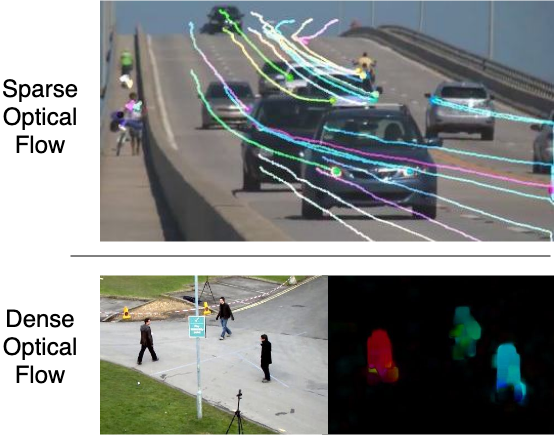
\includegraphics[width=0.80\textwidth]{figures/litsurvey/optical_flow.png}}
    \caption{\label{fig:optical_flow}Visualisation of sparse and dense optical flow algorithms on different shots.}
    \end{figure}
        
    \begin{figure}[h] 
    \centerline{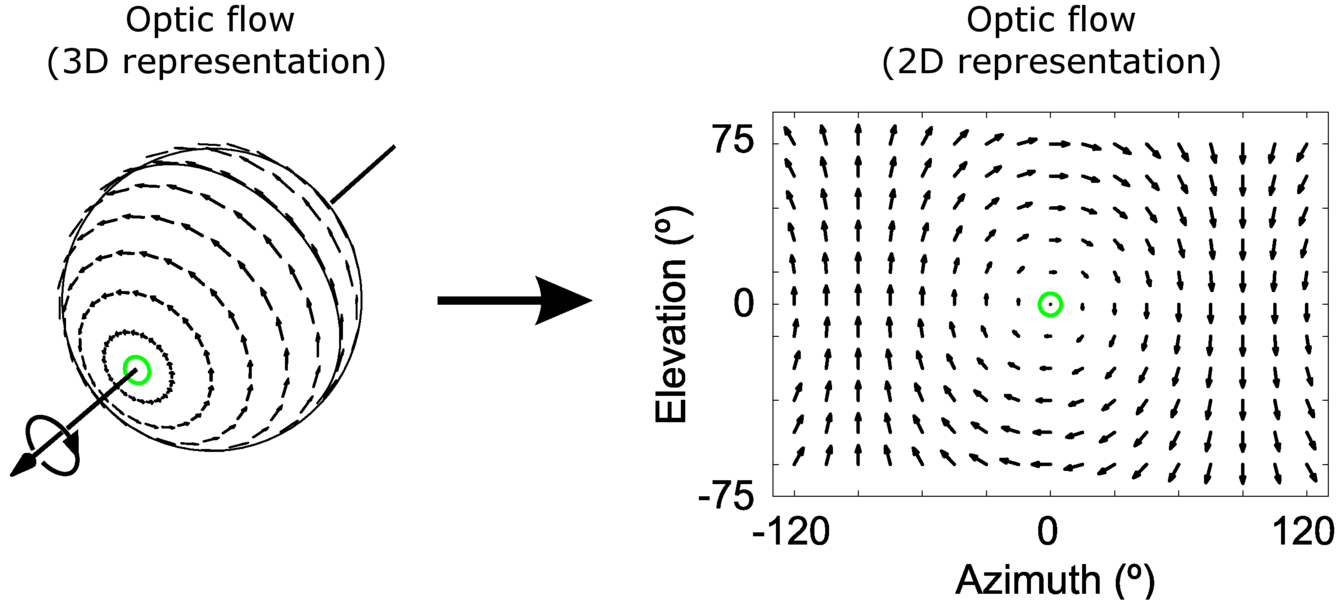
\includegraphics[width=0.80\textwidth]{figures/litsurvey/dense_optical_flow_representation.png}}
    \caption{\label{fig:dense_optical_flow_representation}A 3D and a 2D representation of dense optical flow. Each arrow represents the direction and magnitude of a specific pixel location, which can variate in direction and length.}
    \end{figure}
    
    Object-based motion features have many applications outside of CBVR systems. One of these applications is calculating the optical flow of a shot to prune camera movements caused by unstable recording e.g. hand shaking movement \cite{wang2016actionregonition}. Compared to statistics-based features, trajectory-based features can be used to describe object actions, but they rely on multiple challenging tasks to function efficiently such as correct object tracking and automatic trajectory recording. Finally, object-based motion features can also be classified in a third category: objects' relationship-based motion features. However, these are not described in this literature review as they make use of the objects' symbolic representations, which is not relevant to this topic.
\end{itemize}

% ----------------------------------------------------

\subsection{Learning Models for Pattern Matching}

This section retraces the evolution of pattern matching models, ranging from Bags-of-Visual-Words and Constellation Models to Deep Learning models such as Neural Networks.

\subsubsection{Bag-of-Visual-Words}

The idea of BoVW\footnote{Bag-of-Visual-Words} originates from document analysis, where the frequency words appeared in the text depended on the document type, and the document type could predict the word frequency.\\

Visual words are created by extracting distinctive features such as SIFT, SURF or HoG to train videos from a training set. These features are then clustered using classic models such as Mean-shift or GMMs. The visual words correspond to the middle of each cluster.\\

Histograms can be used by inputting a collection of visual words and a labelled training set of videos. For each video in the dataset, features are extracted and incremented in the related histogram. Once the training is accomplished, a new histogram can be generated for a query video (in a CBVR system) which will then be compared to the previously generated histograms for each dataset video. Example: H. Wang's implementation of BoW histogram \cite{wang2016actionregonition}. Fisher Vectors are an improvement on BoW \cite{araujo2017i2v}.\\

\subsubsection{Constellation Models}

Constellation models are mainly used for detection. Features are organised in space such as a graph model where nodes are labelled with appearance and a Gaussian distribution is present on each node location. There is one model per class, s in a CBVR system, one model per video. The model is moved over image (could be video keyframes), which fires responses at each location. The biggest responses that are larger than a threshold locate the model.

\subsubsection{Deep Learning Models}

\begin{itemize}
    \item Classical Neural Networks
    \item Convolutional Neural Networks
    \item State of the art: AlexNet, VGG, Inception
\end{itemize}


%%%%%%%%%%%%%%%%%%%%%%%%%%%%%%%%%%%%%%%%%%%%%%%%%%%%%%%%%%%%%%%%%%%%%%%%%%%%%%%%%%
% 3 - STRUCTURAL MOVIE PRE-PROCESSING
%%%%%%%%%%%%%%%%%%%%%%%%%%%%%%%%%%%%%%%%%%%%%%%%%%%%%%%%%%%%%%%%%%%%%%%%%%%%%%%%%%
\section{Structural Video Representations}
\label{sec:movie-pre-processing}

The database of videos can be pre-processed to optimise the visual content extraction and pattern matching phases. This section covers different techniques to represent long videos in dense formats, with an emphasis on feature-length movies. As stated in Section \ref{sec:temporal-aspect-videos} on the temporal aspects of videos, movies can be defined as a logically ordered collection of scenes, which contain multiple shots, all made up of individual frames. Shots are therefore the logical fundamental unit to organise and segment a video into \cite{hu2011survey}. Pre-processing the database of movies by segmenting it into a list of shots and representing each shot with a single key frame is a profitable solution that will exponentially improve a CBVR system's efficiency. However, a limit must be set on the amount of data that is segmented to balance the efficiency and the accuracy of the CBVR system.

% ----------------------------------------------------

\subsection{Temporal Movie Segmentation}

The frames that make up a shot usually show strong content correlation. This means that features extracted from one frame will be extremely similar in another frame from the same shot. Detecting shot boundaries would allow the movie to be segmented and organised by shots, as depicted in Figure \ref{fig:shot_boundary_detection}. These boundaries are defined by the type of transition between two different shots, which can either be defined as a quick cut when the transition is direct, or as gradual when it is a dissolve or a fade in/out transition that runs over multiple frames \cite{yuan2007shotboundary}, as shown in Figure \ref{fig:video_transitions}.

\begin{figure}[h] 
\centerline{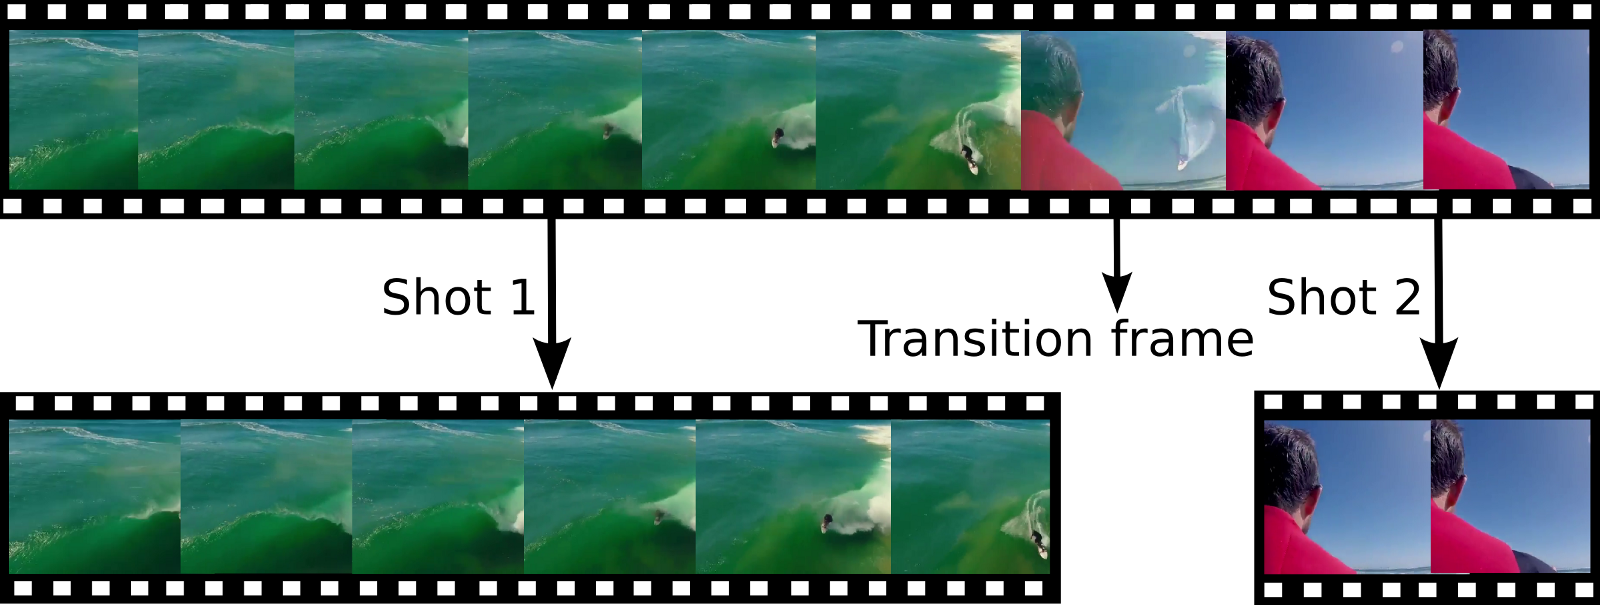
\includegraphics[width=0.75\textwidth]{figures/litsurvey/shot_boundary_detection.png}}
\caption{\label{fig:shot_boundary_detection}Shot boundary detection example of a video scene made up of two shots with a gradual transition between the two shots. Figure courtesy of Michael Gygli available online at: \url{https://medium.com/gifs-ai/ridiculously-fast-shot-boundary-detection-with-fully-convolutional-neural-networks-da9d8c73e86c}}
\end{figure}

\begin{figure}[h] 
\centerline{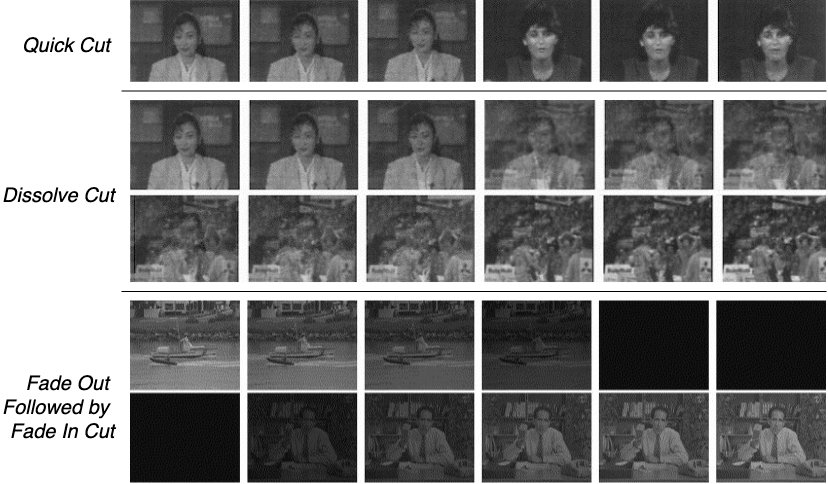
\includegraphics[width=0.75\textwidth]{figures/litsurvey/video_transitions.png}}
\caption{\label{fig:video_transitions}. Visual examples of a quick cut, a dissolve cut and a fading cut. Frames courtesy of Koprinska \& Carrato (2001) ``Temporal video segmentation: A survey'' available online at: \url{https://www.sciencedirect.com/science/article/pii/S0923596500000114}}
\end{figure}

The goal of SBD\footnote{Shot Boundary Detection} is to detect the discontinuity between consecutive frames. Also know as temporal video segmentation, this process requires three steps:
\begin{enumerate}
    \item feature extraction
    \item similarity measurements
    \item shot boundary detection
\end{enumerate}

\subsubsection{Feature Extraction}
\label{sec:feature-extraction-sbd}
The first step in video segmentation consists in extracting features. These features include all the diverse types mentioned in Section \ref{sec:visual-content-extraction}, ranging from static features such as colour-based features (e.g. colour histograms) \cite{hoi2006trecvid06} to dynamic features such as corner points and SIFT\footnote{Scale Invariant Feature Transform}. Although colour histograms are simple to compute and work well with most shots as long as there is at most minor camera movement, they are inefficient when the shots contain major camera movements \cite{hu2011survey}. For example, if in the shot the camera moves from the inside a house towards the outside by going through the window, the frames retrieved from the beginning of the shot will be extremely different to frames from the end of the shot.\\

Dynamic features are therefore more efficient for shot boundary detection than histograms due to their robustness. On the one hand, edge features are more vigorous than histograms when dealing with major camera movement and can handle changes in luminosity. On the other hand, corner and motion features can additionally handle camera motion and the impact of objects in the shot such rapid motion e.g. people walking in front of the camera. However, these dynamic features are more complicated to extract and do not always outperform simple features like colour histograms. Due to their simplicity, colour histograms remain the most common feature extraction technique for shot boundary detection \cite{yuan2007shotboundary}.\\

\subsubsection{Similarity Measurements}
\label{sec:similarity-measurements-sbd}
The second step in video segmentation is to use these extracted features to compute the similarities between frames. Many metrics exist to compute the similarities between two the extracted features. The most basic method consists in computing the Euclidean distance or the absolute distance $g(n,n+k)$ between a pair of frames \cite[p.476]{janwe2013video}, as shown in Equation \ref{eq:absolutevalue}, where $n$ and $n+k$ represent the two frames being compared, and $I_n(x,y)$ the intensity level of frame $n$ at pixels locations $(x,y)$:

\begin{equation}
\label{eq:absolutevalue}
    g(n,n+k) = \sum _{x,y} | I_n(x,y) - I_{n+k}(x,y) |
\end{equation}

More advanced distance metrics can be used based on the type of feature that was extracted. For instance, intersection and chi-square distances can be used to compute the distance between the histograms of two frames \cite[p.197]{camara2007shot}. During the 2006 TRECVID conference, \textit{Hoi et al.}, used grey scale histograms for their extracted features and calculated the colour differences between frames using the EMD\footnote{Earth Mover's Distance}. EMD is used to calculate the distance between two probability distributions, which are represented by the two histograms that represent each frame in \cite[p.2]{hoi2006trecvid06}'s case. These similarities can be measured using two techniques: pair-wise similarities and window similarities.\\

The first technique rests on using pairs of frames to compute the similarities between them. The similarities between two consecutive frames $I_1$ and $I_2$ are compared, before comparing the pair of frames $I_2$ and $I_3$, and so on and so forth until frames $I_{n-1}$ and $I_n$ are compared. This straightforward technique precisely detects rough changes between the visual content in a shot (e.g. quick cuts between two shots) but is more sensitive to intensity changes caused by noise and disturbances such as camera motion and objects, leading to a high level of wrong detections \cite{janwe2013video}.\\

The second technique is the window-based similarity measure, that measures the similarities between multiple frames specified within a range \cite{cernekova2006information}. This helps counter the effects of noise and disturbances captured by the pair-based approach but is more expensive to compute, therefore less used \cite{hu2011survey}.

\subsubsection{Detection}
\label{sec:litsurvey-shot-boundary-detection}

The final step in segmenting a video is the detection of the frames to cut, which is achieved by using the measured similarities between the frames. Two methods exist for this step: a threshold-based approach and a statistical learning-based approach.\\

The \textit{threshold-based approach} compares the measured similarities between a pair of frames with a threshold. Whenever the similarity measure is smaller than the threshold, a shot boundary is detected and the shot can be cut. Figure \ref{fig:shot_boundary_detection_threshold} betrays an example of a threshold-based approach for different types of transitions, with a correct detection (\emph{A}), a missed detection (\emph{B}) and a misinterpreted detection (\emph{C}).\\

\begin{figure}[h] 
\centerline{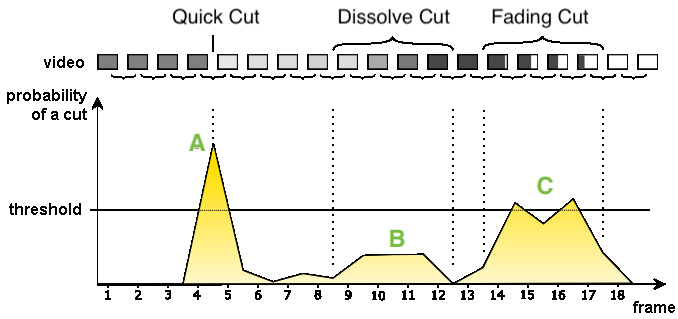
\includegraphics[width=0.75\textwidth]{figures/litsurvey/shot_boundary_detection_threshold.png}}
\caption{\label{fig:shot_boundary_detection_threshold}Threshold-based approach for shot boundary detection. In this example, the shot boundary is detected at \emph{A}, it is missed at \emph{B}, and it is misinterpreted at \emph{C} as two cuts rather than a single one.}
\end{figure}

Either global thresholds, adaptive thresholds, or combinations of both can be used \cite{cernekova2006information} \cite{hu2011survey}:
\begin{itemize}
    \item \textit{Global thresholds} are set empirically and predefined for the entire video. They are therefore inefficient when trying to detect local variations as these are not integrated into the initial global threshold calculations.
    \item \textit{Adaptive thresholds} are local thresholds that are continuously calculated for windows of frames. As the window slides across the video, the threshold is re-estimated accordingly to account for local variations. These are more accurate than global thresholds but are harder to estimate and require some knowledge about the video to set variables such as the window's size.
    \item \textit{Combination of global and adaptive thresholds} are adaptive thresholds that take into account the values of global thresholds when estimating the frames within the window. Different thresholds can be determined for different types of transitions such as cut and dissolve transitions. However, these add increased complexity to the threshold estimation.
\end{itemize}

The \textit{statistical learning-based approach} is a two-class classification task where each frame is classified either as a ``shot change'' or as a ``no shot change'' based on the extracted features and the similarity measurements between those features. In more complex systems, additional classes can be added by adding a classification of quick and gradual transitions for example. Two types of classifiers can be used for this approach:
\begin{itemize}
    \item \textit{Supervised learning-based classifiers}, such as the Support Vector Machine \cite{camara2007shot} and Adaboost \cite[p.617]{zhao2006shot}. These supervised learning approaches have multiple advantages compared to threshold-based approaches as they do not require thresholds to be set and many different types of features can be combined in the feature extraction step to increase the classifier's accuracy. However, this approach requires more expertise as the classifier relies on a well-trained data set to remain accurate \cite{hu2011survey}.
    
    \item \textit{Unsupervised learning-based classifiers} are divided into frame similarity-based and frame-based algorithms. \textit{Frame similarity-based classifiers} groups the similarity measurements between a pair of frames into two clusters. The first cluster holds the similarity measurements with low values, which correspond to the ``shot change'' class, while the second cluster holds the similarity measurements with high values, which correspond to the ``no shot change'' class. K-Means and Fuzzy K-Means clustering algorithms can be used for frame similarity-based classifiers \cite{lo2001fuzzykmeans}. Alternatively, \textit{frame-based classifiers} consider each shot as a cluster of frames with similar features. Clustering ensembles can be used to classify frames into their respective shots \cite{chang2007clusteringensemble}. This approach is advantageous over supervised learning-based classifiers as no prior training is required for, but the logical temporal order of the shots in scenes is not preserved.
\end{itemize}

All the aforementioned techniques in this section that are used in the three steps required in the process of segmenting a video can be applied to feature-length movies but require some improvements to work efficiently with these large videos. For instance, \cite{hanjalic1999moviesegmentation} suggests considering the semantic aspects of movies, since people relate to the story, such as a marking dialogue, when they remember a movie.

% ----------------------------------------------------

\subsection{Key Frame and Thumbnail Extraction}

Frames from the same shot usually describe the same visual content, meaning there is a lot of redundancy amongst the frames that make up a shot. It is therefore more efficient to deal with a single frame that represents the entire shot or the entire video rather than dealing with an entire video.

\subsubsection{Key Frames}

Once shot boundaries have been detected and the video has been divided into a series of shots, a single frame, named the ``key frame'', can be selected to represent the entire shot. \cite{heo2016colortransfer} suggests only considering key frames in videos to operate on. These key frames would be used for all the sections mentioned in this Literature Survey, including the visual content extraction phases, the pattern matching phases, and database videos pre-processing phase. A wide variety of approaches exist to extract a key frame from a video.\\

The most simple approach is \textit{Sequential Comparison Between Frames} where frames are sequentially compared until a frame very different to the previous key frame is found, at which point that frame is set as a new key frame \cite{heo2016colortransfer}. Frames are compared using the features mentioned in Section \ref{sec:feature-extraction-sbd} e.g. histograms, and similarities are calculated using the same distance functions mentioned in Section \ref{sec:similarity-measurements-sbd} e.g. chi-square distance \cite{hu2011survey}. More advanced approaches can be used:

\begin{itemize}
    \item Global Comparison Between Frames
    \item Reference Frame
    \item Clustering
    \item Curve Simplification
    \item Objects/Events
\end{itemize}

To illustrate the advantage of using key frames, a 3-seconds long shot recorded at 30 fps\footnote{Frames Per Second} of a ball rolling on the ground can be used (90 frames in total). Analysing all the frames individually as stills would obviously be highly inefficient. However, selecting key frames to work on, as depicted in Figure \ref{fig:rolling_ball} where a single frame is chosen for each second, would mean that 3 key frames can be used for feature extraction and pattern matching instead of using all of the 90 frames that make up the video.\\

\begin{figure}[h]
\centerline{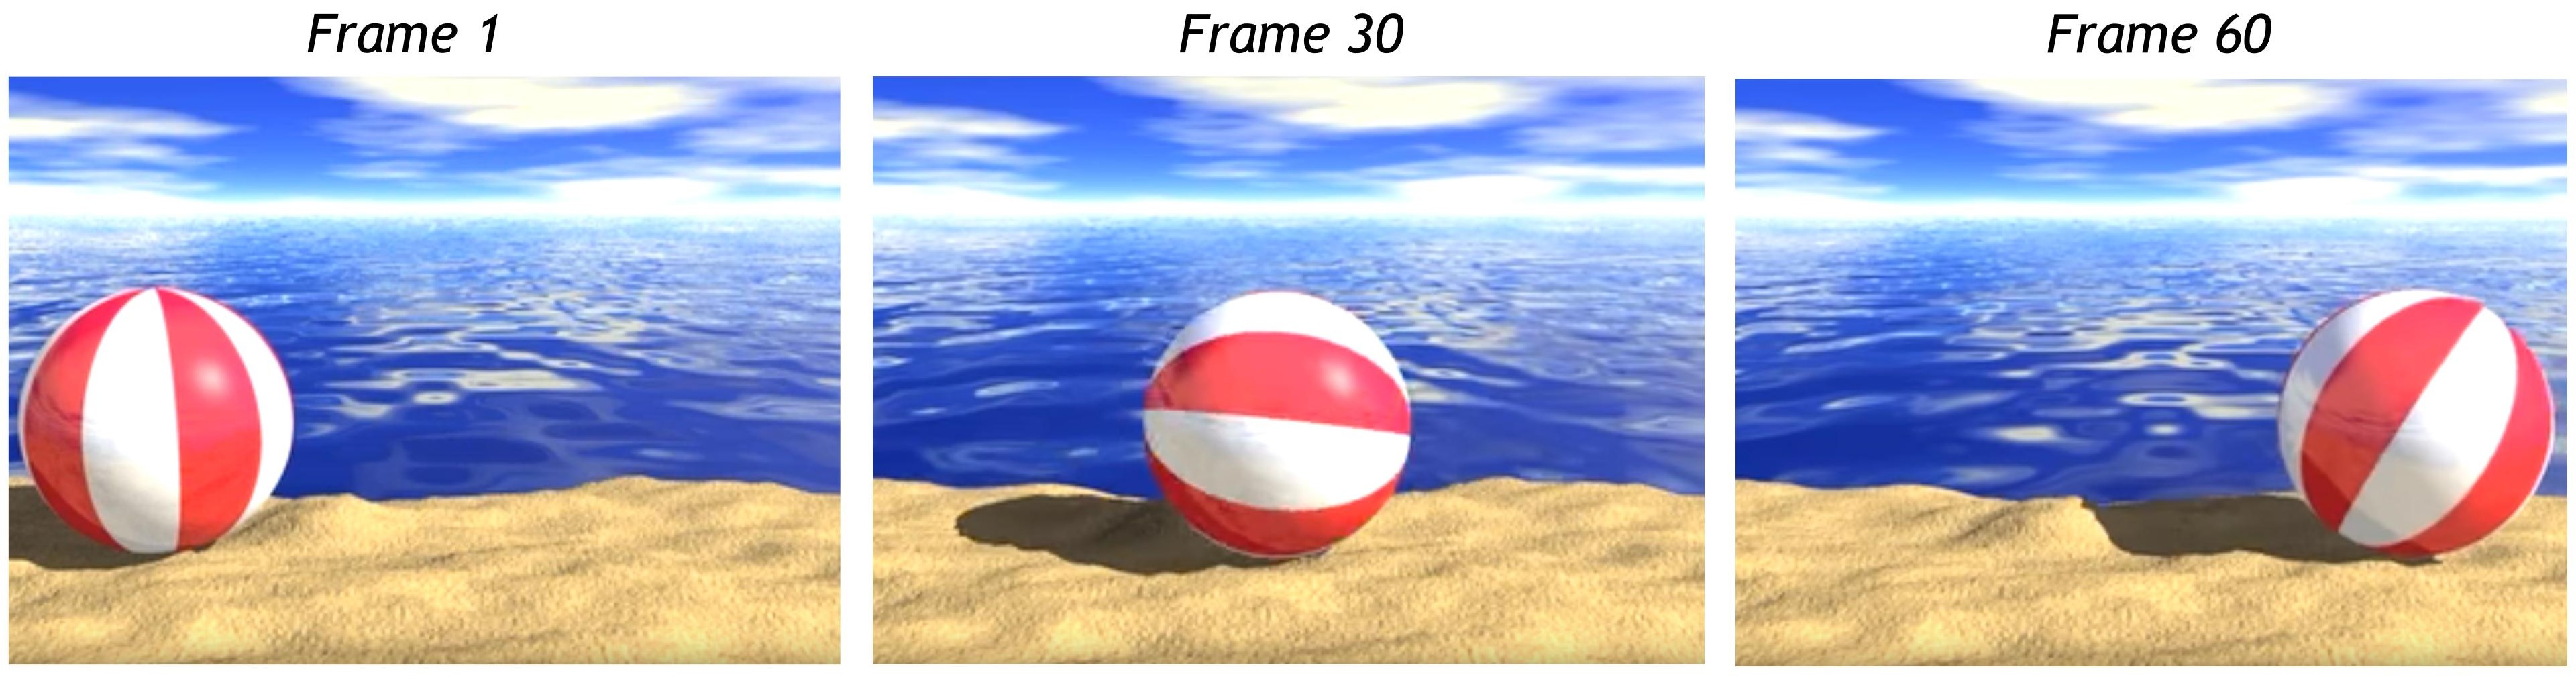
\includegraphics[width=\textwidth]{figures/litsurvey/ball_rolling.jpg}}
\caption{\label{fig:rolling_ball}Example of frames to sample for low-visual content analysis. The first frame for each second (one frame every thirty seconds) is retrieved for a 30 fps 3-second video of a ball rolling from the left-hand side of the screen to the right-hand side. Video frames courtesy of \textit{``How to Animate a Rolling Ball''} YouTube video available online: \url{https://youtu.be/cgbLAreElNI?t=130}.}
\end{figure}

\subsubsection{Thumbnails for Initial Shortlisting}

Thumbnails can be generated for each video in a database, which are stored as additional data along with the original video file \cite{okabe2018animating}. In a CBVR system, the thumbnails for the query video and for the database videos would be generated using the same algorithm in order to create similar outputs. This technique can be used in parallel to \cite{araujo2017i2v}, who states that an initial shortlist of potentially matching videos can be generated before the main pattern matching phase. This shortlist can be created by computing the similarities between the query video's thumbnail and the thumbnails of the database videos.\\

Many advantages can be gained from this small initial step which could have an important impact on the system's overall speed and efficiency performance. Indeed, database videos that share no similarities to the query video will not be considered at all during the main pattern matching phase e.g. if the query video corresponds to a colourful sunset, then database videos of cloudy environments will be immediately filtered out as it is unlikely that they will match with the query video in the main pattern matching phase. This step diminishes the number of videos to compare to the query.\\

This initial step of generating thumbnails for the query video and each video in the database is extremely speedy as it only uses a single frame that describes the entire video. Therefore the entire process will not be noticeably slowed down. However, this concept could only be applied to relatively small databases where the videos contain a single scene with multiple similar shots. Indeed, shots can be characterised by a single still as they are made up of frames with similar visual content, whereas scenes can be made up of shots that change a lot and describe different visual content. Using thumbnails to shortlist a database of feature-length movies would greatly diminish the accuracy of the system due to the high number of scenes that make up a movie that cannot be resumed to a single thumbnail. The database videos' thumbnails will have already been generated during the database's pre-processing phase, which only occurs a single time. A possible solution could be to create a thumbnail for each shot in a scene and store each thumbnail in a list. For example, if a scene contains six different shots, then six thumbnails will be generated to describe that scene.

% ----------------------------------------------------

\subsection{Feature-Length Movie Optimisation}

For quicker pattern matching and feature extraction, 16 pixels separate two feature points, allowing for rough pattern matching rather than exact pattern matching. This could be used when using feature-length movies as database videos to pattern match \cite{okabe2018animating}.\\

Fisher Vectors can be used to generate a compact signature for videos, which will then be used for computing similarities between the query video's FV and the database videos' FVs \cite{araujo2017i2v}.\\


%%%%%%%%%%%%%%%%%%%%%%%%%%%%%%%%%%%%%%%%%%%%%%%%%%%%%%%%%%%%%%%%%%%%%%%%%%%%%%%%%%
% 5 - CHAPTER SUMMARY
%%%%%%%%%%%%%%%%%%%%%%%%%%%%%%%%%%%%%%%%%%%%%%%%%%%%%%%%%%%%%%%%%%%%%%%%%%%%%%%%%%
\section{Chapter Summary}

The literature in this chapter covers the main theoretical and technological aspects required to understand the nature of content-based retrieval systems for videos, how visual content is extracted from these videos and used, and how the temporal structure of videos can be employed for optimisation. With the knowledge gained from the literature coupled with the problems identified in Section \ref{sec:problem-description}, a set of requirements of what the system needs to achieve can be formulated in the next chapter.